% ═══════════════════════════════════════════════════════════════
% MUSTERLÖSUNG: Der Gleichstrommotor (Kl. 9, DS 09a)
% Basiert auf: AB-09a-gleichstrommotor.tex
% ═══════════════════════════════════════════════════════════════

\documentclass[11pt, a4paper]{article}

\usepackage[utf8]{inputenc}
\usepackage[T1]{fontenc}
\usepackage[ngerman]{babel}

% --- SCHRIFTEN ---
\usepackage{helvet}
\renewcommand{\familydefault}{\sfdefault}

\usepackage{microtype}
\usepackage[margin=1.5cm, top=1.8cm, bottom=1.5cm]{geometry}
\usepackage{enumitem}
\usepackage{tabularx}
\usepackage{booktabs}
\usepackage{array}
\usepackage{multicol}
\usepackage{tikz}
\usetikzlibrary{calc,arrows.meta,positioning}

\usepackage{amsmath, amssymb}
\usepackage{siunitx}
\sisetup{locale = DE, per-mode = symbol}

\usepackage{fancyhdr}
\usepackage{lastpage}
\usepackage{needspace}
\usepackage{graphicx}

\usepackage{xcolor}
\usepackage{tcolorbox}
\tcbuselibrary{skins}

% ═══════════════════════════════════════════════════════════════
% FARBEN
% ═══════════════════════════════════════════════════════════════

\definecolor{physik}{HTML}{2c5aa0}
\definecolor{hellgrau}{HTML}{F5F5F5}
\definecolor{mittelgrau}{HTML}{888888}
\definecolor{positiv}{HTML}{C62828}
\definecolor{negativ}{HTML}{1565C0}
\definecolor{magnetisch}{HTML}{2E7D32}
\definecolor{loesung}{HTML}{C62828}

\colorlet{fachfarbe}{physik}

% ═══════════════════════════════════════════════════════════════
% VARIABLEN
% ═══════════════════════════════════════════════════════════════

\newcommand{\fach}{Physik}
\newcommand{\thema}{Der Gleichstrommotor}
\newcommand{\klasse}{9}

% ═══════════════════════════════════════════════════════════════
% KOPF- UND FUSSZEILE
% ═══════════════════════════════════════════════════════════════

\pagestyle{fancy}
\fancyhf{}
\renewcommand{\headrulewidth}{0.4pt}
\renewcommand{\footrulewidth}{0pt}
\lhead{\small \fach{} Klasse \klasse{} | \thema}
\rhead{\small \textcolor{loesung}{\textbf{MUSTERLÖSUNG}}}
\cfoot{\small\textcolor{mittelgrau}{Seite \thepage{} von \pageref{LastPage}}}

% ═══════════════════════════════════════════════════════════════
% BOXEN
% ═══════════════════════════════════════════════════════════════

\newtcolorbox{merkkasten}[1][]{
    colback=hellgrau,
    colframe=hellgrau,
    coltitle=black,
    colbacktitle=hellgrau,
    boxrule=0pt,
    arc=0pt,
    left=8pt, right=8pt, top=6pt, bottom=5pt,
    borderline north={2pt}{0pt}{fachfarbe},
    before skip=5pt, after skip=5pt,
    fonttitle=\bfseries,
    title=#1
}

\newtcolorbox{wortbank}{
    colback=white,
    colframe=fachfarbe,
    boxrule=1pt,
    arc=0pt,
    left=6pt, right=6pt, top=4pt, bottom=4pt,
    before skip=3pt, after skip=3pt
}

% ═══════════════════════════════════════════════════════════════
% BEFEHLE
% ═══════════════════════════════════════════════════════════════

\newcommand{\lsg}[1]{\textcolor{loesung}{\textbf{#1}}}

\setlength{\parindent}{0pt}
\setlength{\parskip}{3pt}

% ═══════════════════════════════════════════════════════════════
% DOKUMENT
% ═══════════════════════════════════════════════════════════════

\begin{document}

% ═══════════════════════════════════════════════════════════════
% HEADER
% ═══════════════════════════════════════════════════════════════

\begin{center}
    {\Large\bfseries\textcolor{fachfarbe}{\thema}}\\[0.15em]
    {\small \textcolor{loesung}{\textbf{Musterlösung}} | \fach{} Klasse \klasse}
\end{center}
\vspace{-0.4em}
\hrule
\vspace{0.5em}

% ═══════════════════════════════════════════════════════════════
% KASTEN 1: AUFBAU
% ═══════════════════════════════════════════════════════════════

\begin{merkkasten}[K1: Aufbau des Gleichstrommotors]

\begin{minipage}{0.48\textwidth}
\textbf{Ordne die Begriffe dem Bild zu:}

\begin{wortbank}
\centering
\textbf{Stator} ~ | ~ \textbf{Rotor} ~ | ~ \textbf{Kommutator} ~ | ~ \textbf{Bürsten} ~ | ~ \textbf{Achse}
\end{wortbank}

\vspace{2mm}
\begin{tabular}{@{}r@{ = }l@{}}
(A) & \lsg{Rotor} \\[0.25em]
(B) & \lsg{Stator} \\[0.25em]
(C) & \lsg{Bürsten} \\[0.25em]
(D) & \lsg{Kommutator} \\[0.25em]
(E) & \lsg{Achse} \\
\end{tabular}
\end{minipage}
\hfill
\begin{minipage}{0.48\textwidth}
\centering
\begin{tikzpicture}
    \node[anchor=south west, inner sep=0] (img) at (0,0)
        {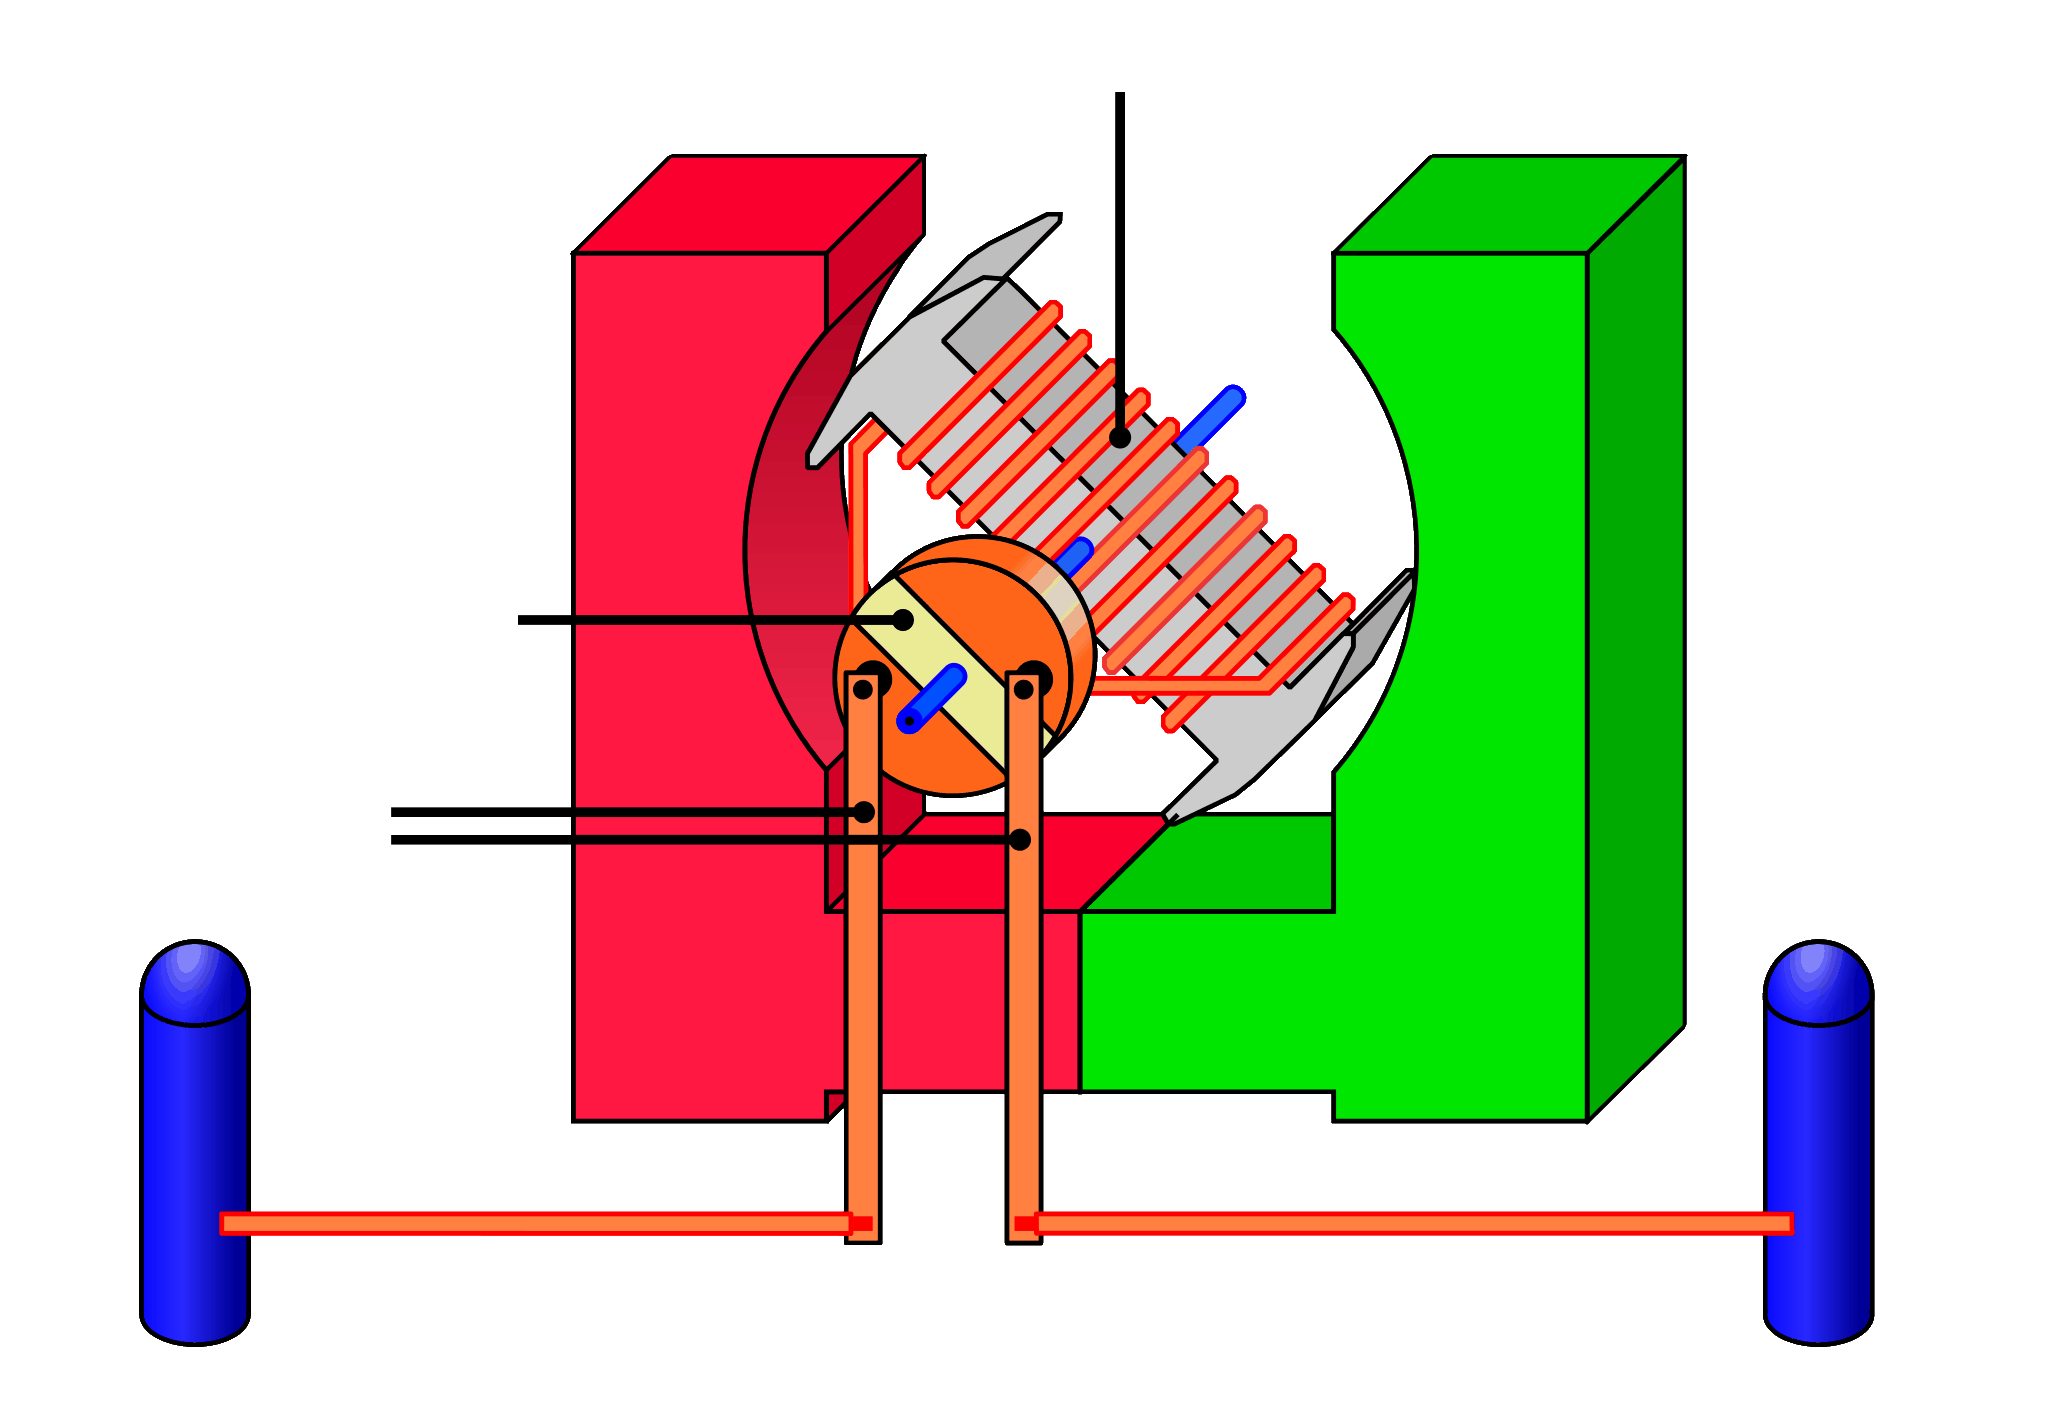
\includegraphics[width=\textwidth]{leifi/img/elektromotor-aufbau-leifi.png}};
    \begin{scope}[x={(img.south east)}, y={(img.north west)}]
        \node[fill=white, draw=black, thick, font=\footnotesize\bfseries] at (0.48, 0.77) {(A)};
        \node[fill=white, draw=black, thick, font=\footnotesize\bfseries] at (0.70, 0.65) {(B)};
        \node[fill=white, draw=black, thick, font=\footnotesize\bfseries] at (0.12, 0.50) {(C)};
        \node[fill=white, draw=black, thick, font=\footnotesize\bfseries] at (0.18, 0.63) {(D)};
        \node[fill=white, draw=black, thick, font=\footnotesize\bfseries] at (0.545, 0.98) {(E)};
    \end{scope}
\end{tikzpicture}\\[1mm]
{\tiny Quelle: LEIFIphysik (CC BY-NC 4.0)}
\end{minipage}

\end{merkkasten}

% ═══════════════════════════════════════════════════════════════
% KASTEN 2: LORENTZKRAFT
% ═══════════════════════════════════════════════════════════════

\begin{merkkasten}[K2: Lorentzkraft -- Kraft auf stromdurchflossene Leiter]

\begin{minipage}{0.58\textwidth}
\textbf{Merksatz:}\\
Ein stromdurchflossener Leiter im \textcolor{magnetisch}{\textbf{Magnetfeld}} erfährt eine \textbf{Kraft} -- die \textbf{Lorentzkraft}.

\vspace{2mm}
\textbf{Richtung der Kraft bestimmen:}\\
Die Kraft steht \textbf{senkrecht} zu:
\begin{itemize}[noitemsep, leftmargin=*]
    \item der \textcolor{positiv}{\textbf{Stromrichtung}} (technisch: + $\rightarrow$ $-$)
    \item dem \textcolor{magnetisch}{\textbf{Magnetfeld}} (N $\rightarrow$ S)
\end{itemize}

\vspace{2mm}
\textbf{Aufgabe:} Zeichne den \textbf{Kraftpfeil} ($\vec{F}$) ein!\\
\lsg{$\rightarrow$ Kraft zeigt nach oben (aus der Seite heraus)}
\end{minipage}
\hfill
\begin{minipage}{0.38\textwidth}
\centering
\begin{tikzpicture}
    \node[anchor=south west, inner sep=0] (img) at (0,0)
        {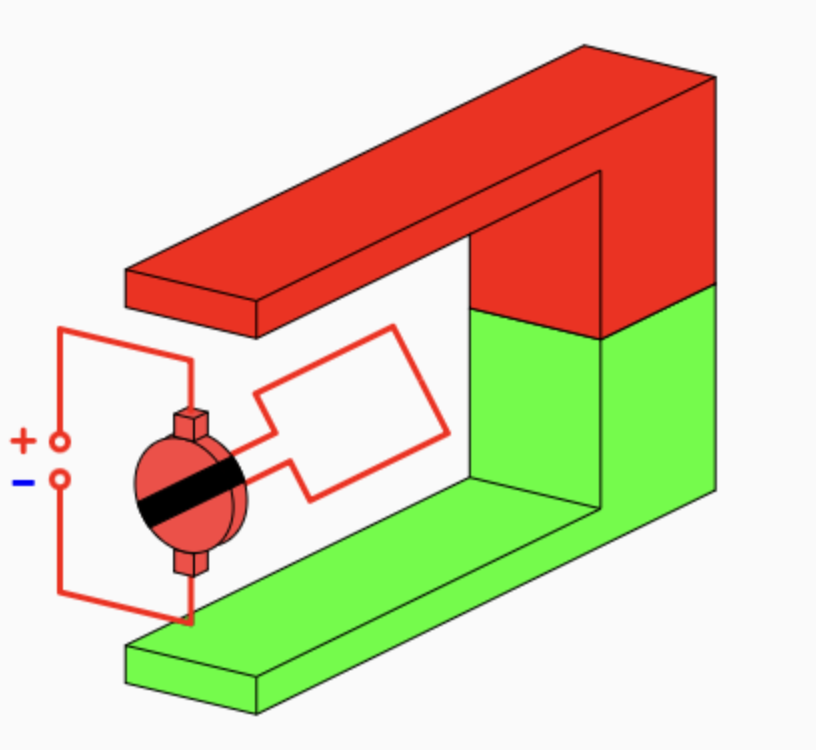
\includegraphics[width=0.95\textwidth]{leifi/img/fendt-45grad.png}};
    \begin{scope}[x={(img.south east)}, y={(img.north west)}]
        \fill[white] (-0.04,0.30) rectangle (0.06,0.54);
        \node[font=\bfseries\large] at (0.01,0.46) {\textcolor{negativ}{$-$}};
        \node[font=\bfseries\large] at (0.01,0.36) {\textcolor{positiv}{$+$}};
        % Kraftpfeil eingezeichnet
        \draw[-{Stealth[length=3mm]}, line width=1.5pt, color=loesung] (0.5,0.55) -- (0.5,0.85);
        \node[font=\bfseries, color=loesung] at (0.62,0.70) {$\vec{F}$};
    \end{scope}
\end{tikzpicture}\\[1mm]
{\tiny Simulation: W. Fendt (Pole vertauscht)}

\vspace{2mm}
\textcolor{positiv}{$\longrightarrow$ Stromrichtung (I)}\\
\textcolor{magnetisch}{$\longrightarrow$ Magnetfeld (B)}
\end{minipage}

\end{merkkasten}

% ═══════════════════════════════════════════════════════════════
% KASTEN 3: ROTOR ALS ELEKTROMAGNET
% ═══════════════════════════════════════════════════════════════

\begin{merkkasten}[K3: Der Rotor als Elektromagnet]

\textbf{Wichtige Erkenntnis:}\\
Der stromdurchflossene Rotor ist selbst ein \lsg{Elektromagnet}!

Er hat einen \textbf{Nordpol (N)} und einen \textbf{Südpol (S)}.

\vspace{3mm}
\begin{minipage}{0.48\textwidth}
\textbf{Magnetische Wechselwirkung:}
\begin{itemize}[noitemsep, leftmargin=*]
    \item N--S: \lsg{ziehen sich an}
    \item N--N oder S--S: \lsg{stoßen sich ab}
\end{itemize}
\end{minipage}
\hfill
\begin{minipage}{0.48\textwidth}
\textbf{Warum dreht sich der Rotor?}\\
Der \textcolor{positiv}{N}-Pol des Rotors wird vom \textcolor{negativ}{S}-Pol des Stators \lsg{angezogen}.
\end{minipage}

\vspace{3mm}
{\small\textit{$\rightarrow$ Schau dir die Animation im Lernpfad an!}}

\end{merkkasten}

% ═══════════════════════════════════════════════════════════════
% KASTEN 4: KOMMUTATOR + ENERGIE
% ═══════════════════════════════════════════════════════════════

\begin{merkkasten}[K4: Der Kommutator -- Warum der Motor weiterdreht]

\textbf{Das Problem:}\\
Der N-Pol des Rotors wird zum S-Pol des Stators gezogen -- und bleibt dort \lsg{stehen}!\\
{\small (nach kurzem Pendeln)}

\vspace{2mm}
\textbf{Die Lösung -- Der Kommutator:}\\
Der Kommutator \lsg{wechselt / kehrt um} die Stromrichtung im Rotor genau im richtigen Moment.\\
$\Rightarrow$ Die Pole des Rotor-Elektromagneten werden \lsg{umgepolt}.\\
$\Rightarrow$ Jetzt wird er wieder \lsg{abgestoßen} und dreht weiter!

\vspace{3mm}
\begin{minipage}{0.48\textwidth}
\textbf{Energieumwandlung im Motor:}

\vspace{3mm}
\centering
\begin{tikzpicture}[node distance=0.8cm, every node/.style={font=\small}]
    \node[draw, fill=hellgrau, minimum width=2.2cm, minimum height=0.8cm] (ein) {\lsg{Elektrische}};
    \node[right=of ein, font=\Large] (pfeil) {$\rightarrow$};
    \node[draw, fill=hellgrau, minimum width=2.2cm, minimum height=0.8cm, right=of pfeil] (aus) {\lsg{Bewegungs-}};
    \node[above=0.1cm of ein, font=\tiny] {Energie};
    \node[above=0.1cm of aus, font=\tiny] {Energie};
\end{tikzpicture}
\end{minipage}
\hfill
\begin{minipage}{0.48\textwidth}
\centering
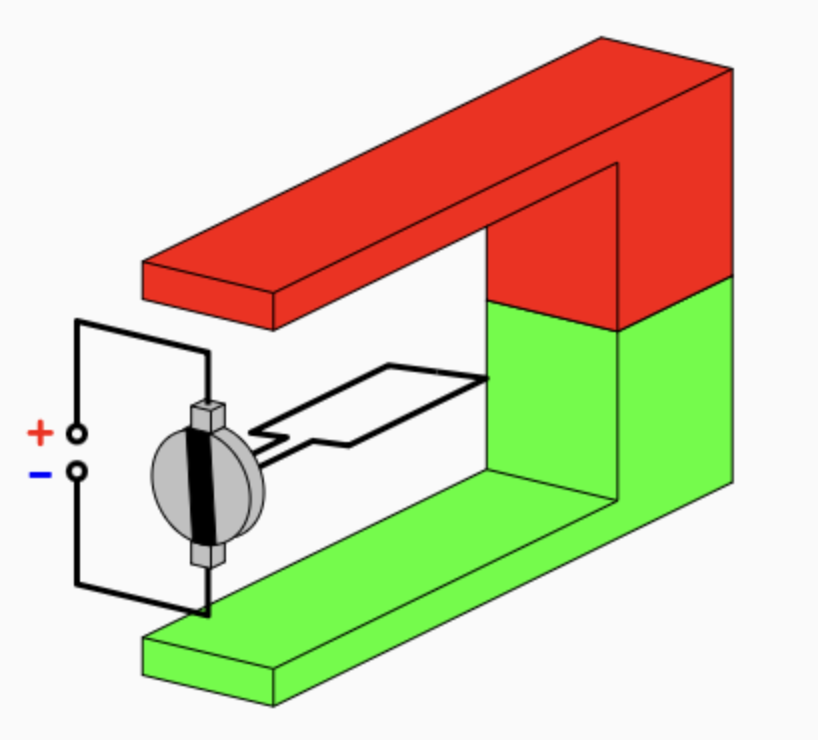
\includegraphics[width=0.85\textwidth]{leifi/img/fendt-horizontal.png}\\
{\tiny Totpunkt: Hier schaltet der Kommutator um!}
\end{minipage}

\end{merkkasten}

% ═══════════════════════════════════════════════════════════════
% KASTEN 5: DREHRICHTUNG ÄNDERN
% ═══════════════════════════════════════════════════════════════

\begin{merkkasten}[K5: Drehrichtung des Motors ändern]

\textbf{Die Drehrichtung kann geändert werden durch:}

\vspace{2mm}
\begin{tabularx}{\textwidth}{|X|c|}
\hline
\textbf{Methode} & \textbf{Drehrichtung ändert sich?} \\
\hline
Spannung umpolen (+ und $-$ vertauschen) & \lsg{$\boxtimes$ Ja} \quad $\square$ Nein \\
\hline
Magnetfeld umpolen (N und S vertauschen) & \lsg{$\boxtimes$ Ja} \quad $\square$ Nein \\
\hline
\textbf{Beides gleichzeitig} ändern & $\square$ Ja \quad \lsg{$\boxtimes$ Nein} \\
\hline
\end{tabularx}

\vspace{3mm}
\textbf{Begründung} (ein Satz):

\vspace{2mm}
\lsg{Wenn man beides gleichzeitig ändert, heben sich die beiden Änderungen auf -- die Drehrichtung bleibt gleich.}

\end{merkkasten}

% ═══════════════════════════════════════════════════════════════
% FUSSZEILE
% ═══════════════════════════════════════════════════════════════

\vfill

\begin{center}
\small\textcolor{mittelgrau}{Dieses AB begleitet den Lernpfad LP-09a. Nach Bearbeitung: Minitest MT-09a.}
\end{center}

\end{document}
